作成したプログラムをリスト\ref{fish_newral.py}に示す.
今回は,トレーニングデータAとBを読み込んでラベル付け
を行い,シャフルしトレーニングデータとテストデータに分けた.
ネットワークは,XORと同様のものを使い,1,0での分類を行った.

fishの学習がうまく行っていることをテストデータで確認
した.テストデータでは,$\frac{9}{10}$(90%)の精度を
記録した.

学習過程の誤差の変化を図\ref{error-2}に示す.

\begin{figure}[htb]
  \centering
  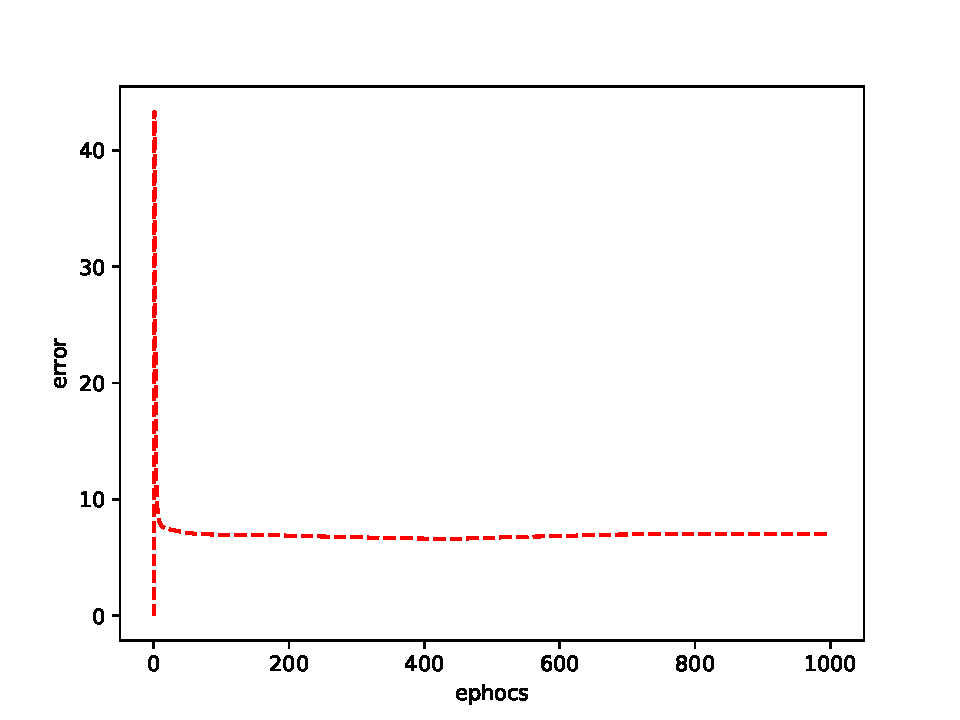
\includegraphics[scale=0.5]{img/error2.pdf}
  \caption{fishA,B学習時の誤差変化}
  \label{error-2}
\end{figure}
